\documentclass[]{article}
\usepackage[UTF8]{ctex}
\usepackage[top=2.5cm, bottom=2cm, left=2.5cm, right=2.5cm]{geometry}
\usepackage{url}
\usepackage{graphicx}
\usepackage{float}
\usepackage{cite}
\usepackage{fancyhdr}
\usepackage{multicol}

\pagestyle{fancy}
\setlength{\parindent}{2pt} % 设置开头的缩进
% 更改摘要和关键词标题为英文
\renewcommand{\abstractname}{Abstract}
% 添加关键词命令
\newcommand{\keywords}[1]{\textbf{Keywords:} #1}
%opening
\title{容错的分布式键值存储系统}
\author{刘芳新\\ \footnotesize 中山大学~~智能科学与技术~~21312482}
\date{\today}
\begin{document}
	\maketitle
	\thispagestyle{fancy} % 仅在标题页使用自定义的页眉设置
	\vfill
	\hrule
	\footnotesize
	\vspace{12pt} % 插入12点的垂直空间
	\begin{minipage}{\textwidth}
		\raggedright % 左对齐
		学号: 21312482 \\ 
		课程: 分布式计算实验 \\ 
		日期:\today \\ 
		Email:liufx7@mail2.sysu.edu.cn
	\end{minipage}
	\normalsize 
	\newpage % 分页命令
	\tableofcontents % 生成目录页
	\newpage % 分页命令
	\section{lab3-A kv server}
	\subsection{任务分析}
	Lab 3A的任务是在之前实现的Raft算法的基础上构建一个基于Raft的键值存储服务器(KV server)。这样的服务器可以提供分布式的键值存储服务,并通过Raft算法确保数据的一致性。以下是对Lab 3A的任务的分析:
	\begin{itemize}
	\item KV Server: 需要实现一个简单的键值存储服务器,支持基本的键值对操作,如读取(Get)、写入(Put)、修改(Append)等。这个服务器将在多个节点上运行,通过Raft算法维护数据的一致性。
	\item Raft集成: KV服务器将使用之前实现的Raft算法来确保在分布式环境下数据的一致性。每个KV服务器节点都是Raft节点,参与领导者选举、日志复制、一致性维护等Raft算法的操作。
	\item 客户端请求处理: KV服务器需要能够处理来自客户端的键值操作请求。这可能涉及到网络通信、请求解析、操作执行等。
	\item 状态机和数据存储: KV服务器作为Raft的状态机,需要维护键值对的状态。你需要实现数据的存储和管理,确保数据在节点之间正确地复制和同步。
	\end{itemize}

	\subsection{common功能设计}
	公共部分需要完善PutAppendArgs和GetArgs结构体,我在这两个结构体中额外添加了Id属性,用来标识这个独一无二的请求,避免重复执行。
	\subsection{client功能设计}
	客户端需要向服务器发送请求。
	\subsubsection{完善Clerk结构体}
	Clerk结构体就是客户端,在这其中,我添加了三个字段:leader、peerNum和name。
	
	\begin{itemize}
		\item leader字段: 用于存储搜索到的领导者的索引。这个字段对于了解当前网络中的领导者是非常有用的。
		\item peerNum字段: 记录了服务器的数量。通过这个字段,我们可以知道整个系统中有多少个节点,这对于一致性算法的正常运行是必要的信息。
		\item name字段: 用于标识客户端。通过这个字段,我们可以清晰地辨识和区分不同的客户端,这在处理多个客户端请求时非常重要。
	\end{itemize}
	\subsubsection{完善MakeClerk函数}
	MakeClerk 创建并返回一个 Clerk 客户端,当客户端刚刚启动时,由于还不知道领导者的位置,因此将leader字段设置为-1。这是一种合理的初始化,表示客户端在开始时对领导者的位置没有具体信息。
	\subsubsection{完善Get函数}
	客户端在发起 Get 请求时,首先需要检查当前是否已确认领导者。如果领导者为 -1,客户端需要通过轮询遍历的方式搜索新的领导者。这种搜索方式虽然直接简单,但由于 Raft 复制的数量通常不会很多,因此一次轮询的性能开销较小。
	
	Get 请求的 RPC 参数应包含 Key 和一个 Id。
	
	在客户端和服务端之间的交互中可能会遇到一些问题,考虑了以下几种情况:
	\begin{itemize}
		\item Consensus Error(共识错误): 表示服务端对该请求的共识过程发生错误,无法完成共识,因此无法执行该请求。可能原因是请求的服务端不再是合法的 leader,或者是 Raft 集群出现问题。客户端的处理措施是重新进行搜索,寻找另一个 leader。这种方式直观地解决了第一种情况,如果是第二种情况,客户端会重新搜索到相同的 leader 并再次尝试请求,直到 Raft 集群恢复。
		\item Not Leader(非领导者错误): 表示一个非 leader 的服务端接收到了客户端的请求。客户端需要重新向下一个服务器尝试发起请求。
		\item RPC 请求无法到达服务器: 表示网络出现问题,无法和服务器建立连接进行 RPC 请求。客户端应该向下一个服务器尝试发起请求。
	\end{itemize}
	\subsubsection{完善PutAppend函数}
	原理和Get函数同理,唯一的区别就是返回值的差别。PutAppend函数的返回值中没有value值。
	\subsection{server功能设计}
	服务器端需要接受请求,并通过底层Raft来保持log的一致性,操作存储在内存中。
	\subsubsection{完善Op结构体}
	这个Op结构体用于给我们服务端的简单数据库进行执行请求用的,同时,这个结构体也被用作命令,发送到 Raft 中进行共识。
	
	\subsubsection{完善KVServer结构体}
	KVServer表示键值储存服务器,我添加了以下字段:
	\begin{itemize}
		\item CommandLog:是一个映射型的数据结构,专门用于存储已经执行过的请求的 Id 值。其设计采用了 map 这个数据类型,以请求的 Id 为 key。这个变量的主要作用是提供一种快速查找的机制,用于判断某个指令 Id 是否已经有执行记录。
		\item CommandLogQueue:则是一个队列,用于追踪记录最近的几条请求。在进行快照时,需要将最近的请求记录保存在这个队列中。这样设计的目的是确保在服务端重启后,系统能够迅速恢复并回复那些最近可能发生的重复请求,从而保持数据的一致性。
		\item cond:一个条件变量,它被设计用于后续的同步执行。
		\item Data:一个代表简单数据库的变量,用于存储指令的执行结果。
	\end{itemize}
	
	\subsubsection{完善Get函数}
	服务端在接收到客户端的请求后,首先通过 kv.CommandLog 判断该请求是否为重复请求,即是否已经有记录。如果是重复请求,则直接返回上次执行的结果。
	
	对于非重复请求,服务端将 RPC 参数封装为 Op 结构体,作为命令传递给 Raft 模块进行共识。调用 Start 函数开始对该请求进行 Raft 共识。在这个过程中,需要考虑几种情况:
	\begin{itemize}
		\item 如果 Start 函数返回本节点非 leader,服务端返回错误信息:“Not leader”。
	
		\item 如果 Start 函数返回本节点为 leader,服务端将开启一个计时器协程,并阻塞等待请求的共识完成并成功执行。如何判断是否共识成功并执行呢?每当有一条请求共识成功并进入 applyCh 中,由 executeThread 线程进行执行,这时会唤醒等待的线程。被唤醒的线程判断是否为自己负责的请求,如果不是,则继续阻塞。这里可能有两种情况:(1)共识成功并成功执行;(2)本节点由于网络分区已经是过时的 leader,始终无法完成请求的共识成功。如果计时器超时后仍未完成,则返回错误信息:“Consensus error”。
	
		\item 如果完成 Raft 共识后,服务端等待该请求的执行。通过开启一个协程 executeThread 来监控 applyCh 管道中的请求,并执行管道中的请求。每有一条请求被执行,Get 函数都会查看是否为本请求被成功执行。若成功执行,则查看执行结果并返回。
	\end{itemize}
	\par
	在 KVServer 结构体中,设计了一个 cond 条件变量用于协调 executeThread 协程和 Get 协程。Get 协程在发现本请求成功共识后,会阻塞等待该请求是否被及时执行。而 executeThread 协程在每次执行完一条指令后,都会唤醒所有等待本请求执行结束的协程,使它们检查是否自己的请求被执行成功,若成功则返回结果给客户端。
	
	\subsubsection{完善PutAppend函数}
	逻辑和Get函数一模一样,此处不赘述。
	
	\subsubsection{设计executeThread函数}
	executeThread 函数是 KV 服务器中一个关键的处理函数,它处理 Raft 模块传递过来的 ApplyMsg。以下是 executeThread 函数的详细原理:
	\begin{enumerate}
	    \item executeThread 是一个无限循环的 goroutine,它持续监听 applyCh 通道,该通道由 Raft 模块用于传递已经提交的日志条目(命令)。
	
	    \item 当有新的日志条目被提交时,executeThread 会从 applyCh 中接收到一个 ApplyMsg 对象。
	
	    \item 如果 ApplyMsg 中的 SnapshotValid 字段为 true,说明这是一个快照(snapshot),executeThread 会解码快照中的数据,包括键值对的状态和已经执行的命令日志。然后将这些数据恢复到 KV 服务器的状态中。
	
	    \item 如果 ApplyMsg 中的 CommandValid 字段为 true,说明这是一个客户端的命令。executeThread 提取出命令中的操作类型(Get、Put、Append)和相应的参数,然后执行相应的操作。
		\begin{itemize}
	        \item 对于 Get 操作,executeThread 从服务器状态中获取相应的值,将其放入命令结果中,并将结果保存到命令日志中,供后续查询使用。
	
	        \item 对于 Put 操作,executeThread 更新服务器状态中的键值对,并将结果保存到命令日志中。
	
	        \item 对于 Append 操作,executeThread 将指定键的值追加指定内容,并将结果保存到命令日志中。
		\end{itemize}
	    \item 执行完命令后,executeThread 会通过条件变量 cond 发送信号通知可能在等待的线程,以便它们能够获取最新的状态或者获取相应的命令结果。
	
	    \item 这个循环不断地处理新的提交,确保服务器状态与 Raft 模块的日志保持一致。由于 applyCh 中的消息是有序的,因此 KV 服务器能够按照提交的顺序正确执行每个命令。
	\end{enumerate}
	
	\subsubsection{完善StartKVServer函数}
	在这里,我添加了我之前额外引入的一些变量和函数。
	
	kv.CommandLog、kv.CommandLogQueue、kv.cond、kv.Data 都进行了初始化,并开启一个线程执行 executeThread 函数,以实时监控 applyCh 管道并执行其中的请求。
	
	\subsection{代码实现}
	\begin{itemize}
		\item 公共部分
		\begin{figure}[H]
			\centering
			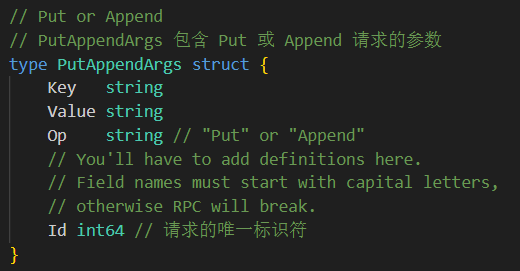
\includegraphics[width=0.8\textwidth]{./3A/PutAppendArgs.png}
			\caption{PutAppendArgs结构体}
		\end{figure}
		\begin{figure}[H]
			\centering
			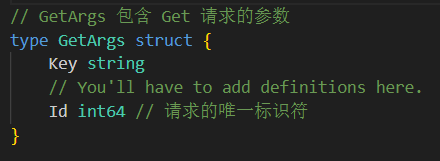
\includegraphics[width=0.8\textwidth]{./3A/GetArgs.png}
			\caption{GetArgs结构体}
		\end{figure}
		\item 客户端部分
		\begin{figure}[H]
			\centering
			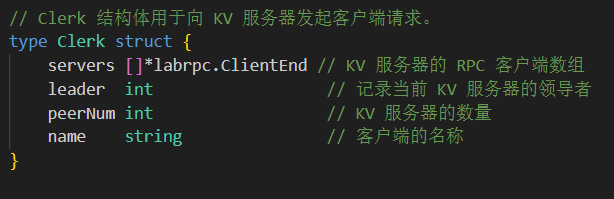
\includegraphics[width=0.8\textwidth]{./3A/Clerk.png}
			\caption{Clerk结构体}
		\end{figure}
		\begin{figure}[H]
			\centering
			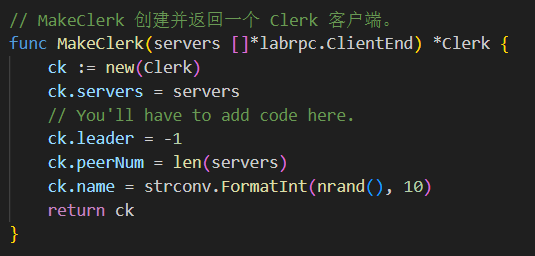
\includegraphics[width=0.8\textwidth]{./3A/MakeClerk.png}
			\caption{MakeClerk函数}
		\end{figure}
		\begin{figure}[H]
			\centering
			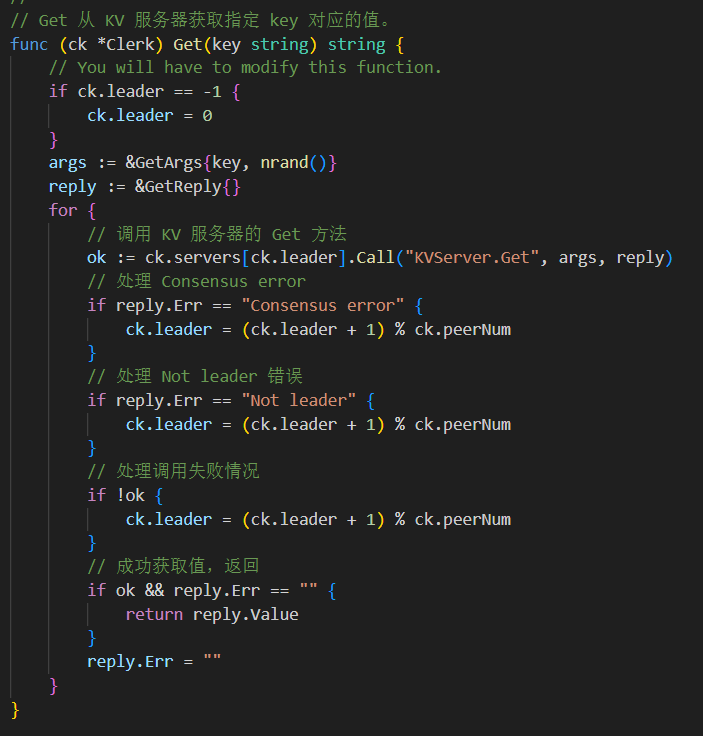
\includegraphics[width=0.8\textwidth]{./3A/client-Get.png}
			\caption{Get函数}
		\end{figure}
		\begin{figure}[H]
			\centering
			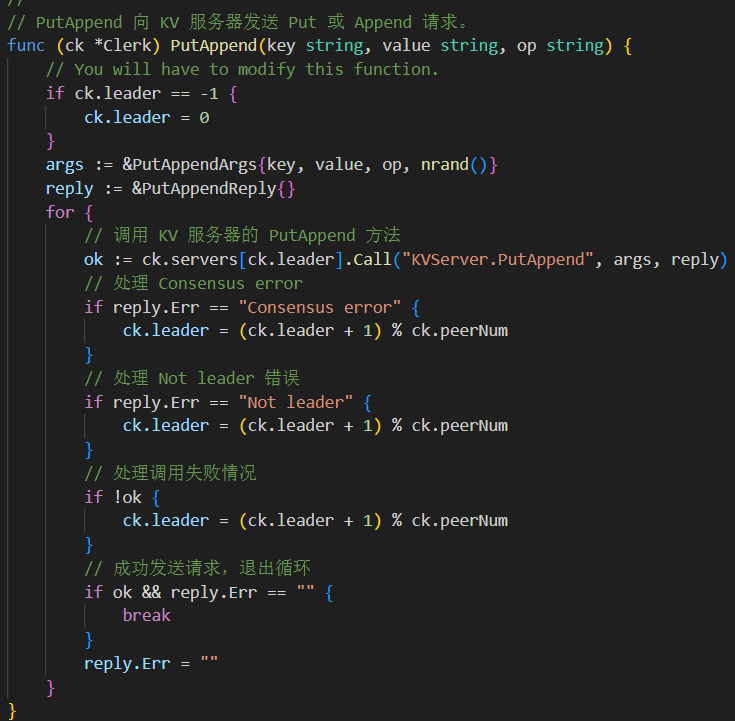
\includegraphics[width=0.8\textwidth]{./3A/client-PutAppend.png}
			\caption{PutAppend函数}
		\end{figure}
		\item 服务器端部分
		\begin{figure}[H]
			\centering
			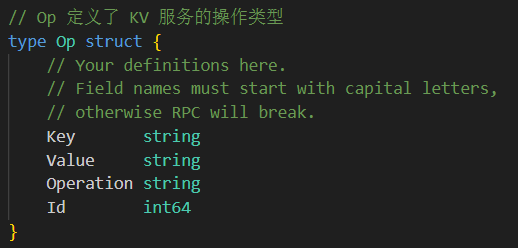
\includegraphics[width=0.8\textwidth]{./3A/Op.png}
			\caption{Op结构体}
		\end{figure}
		\begin{figure}[H]
			\centering
			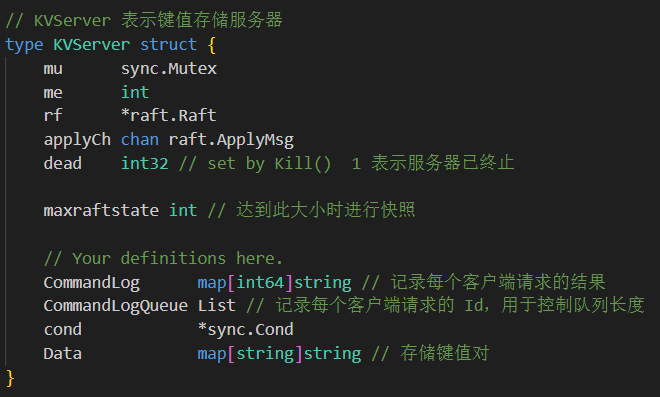
\includegraphics[width=0.8\textwidth]{./3A/KVServer.png}
			\caption{KVServer结构体}
		\end{figure}
		\begin{figure}[H]
			\centering
			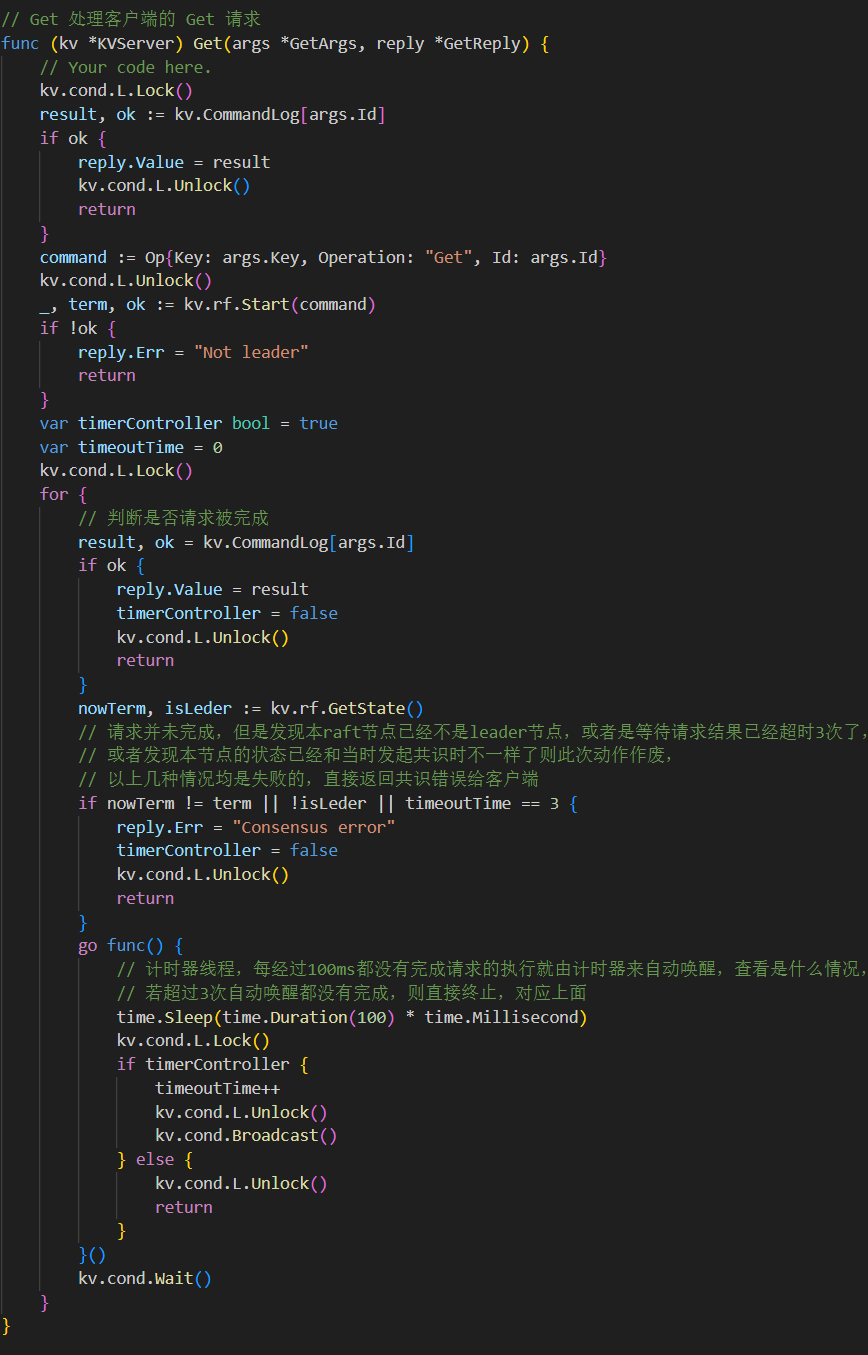
\includegraphics[height=0.95\textheight]{./3A/server-Get.png}
			\caption{Get函数}
		\end{figure}
		\begin{figure}[H]
			\centering
			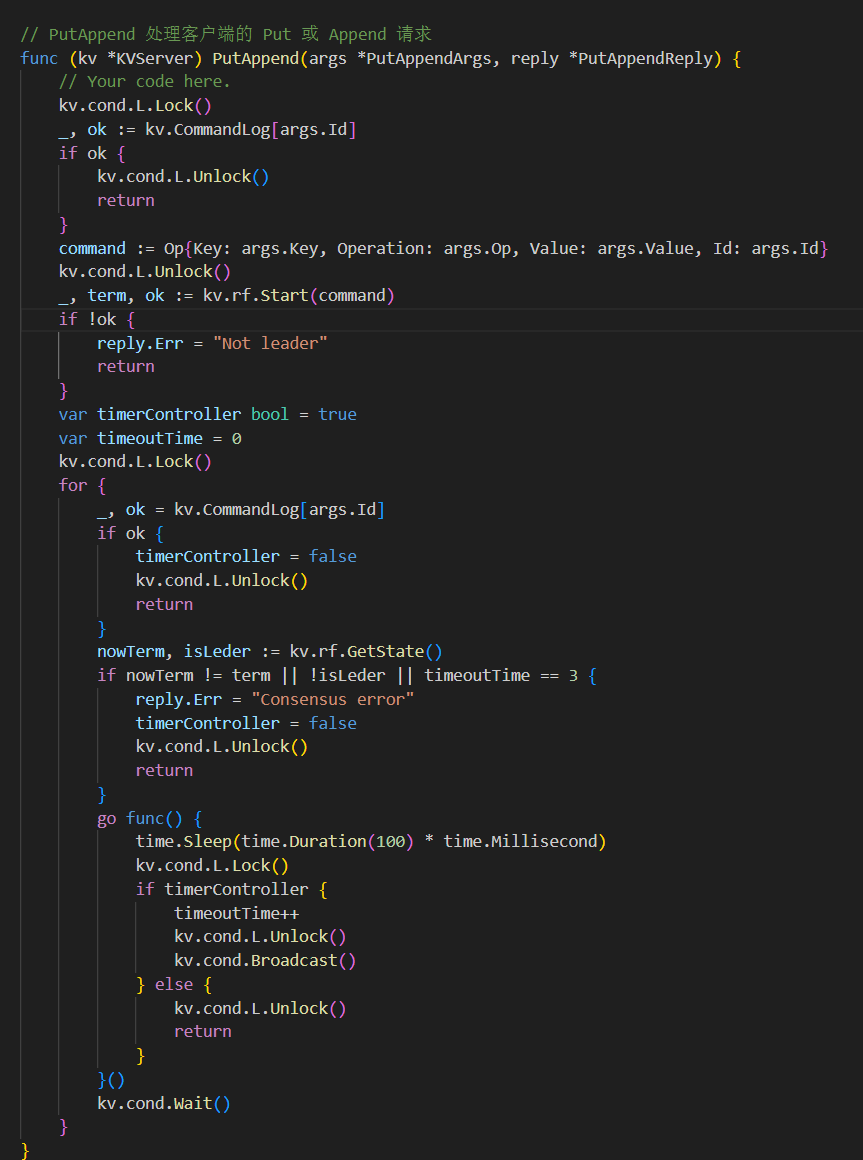
\includegraphics[height=0.95\textheight]{./3A/server-PutAppend.png}
			\caption{PutAppend函数}
		\end{figure}
		\begin{figure}[H]
			\centering
			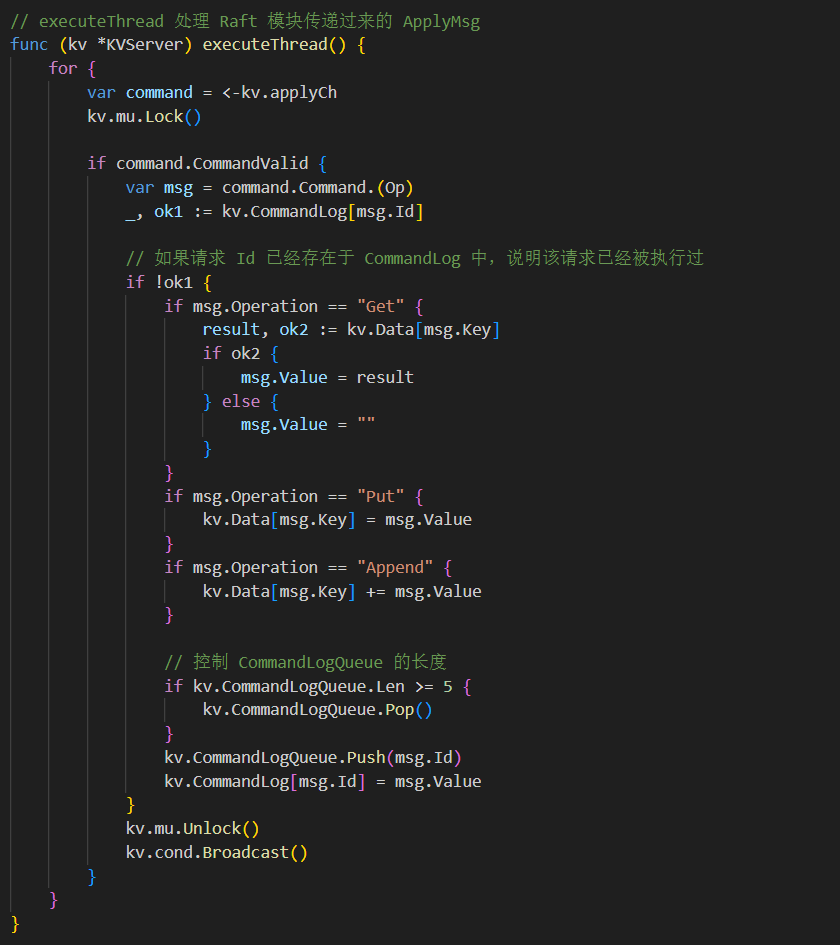
\includegraphics[width=0.95\textwidth]{./3A/executeThread.png}
			\caption{executeThread函数}
		\end{figure}
		\begin{figure}[H]
			\centering
			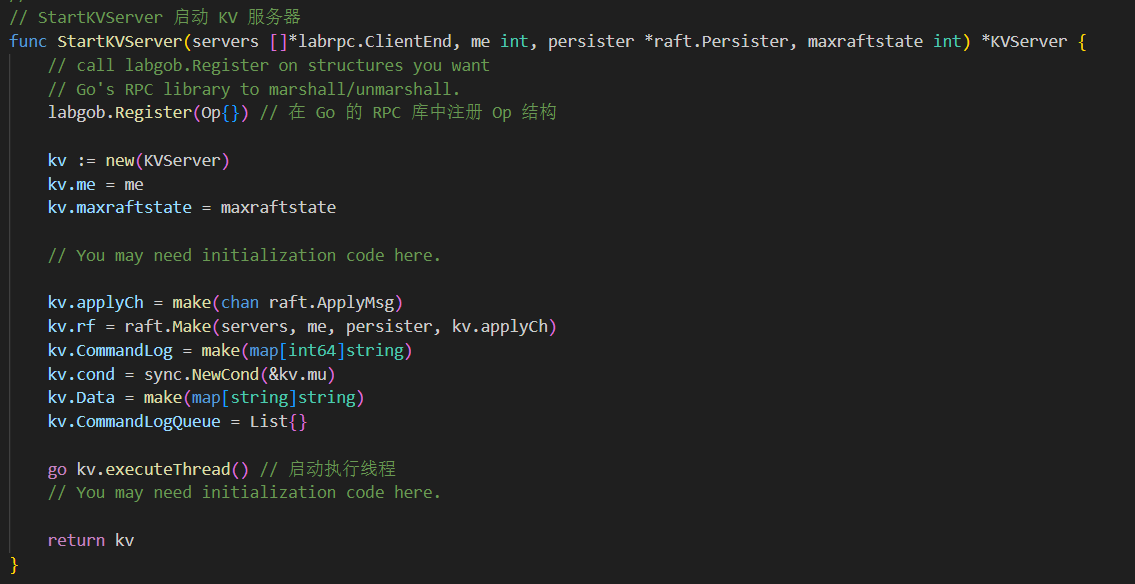
\includegraphics[width=0.8\textwidth]{./3A/StartKVServer.png}
			\caption{StartKVServer函数}
		\end{figure}
	\end{itemize}

	\subsection{测试结果}
	\begin{figure}[H]
		\centering
		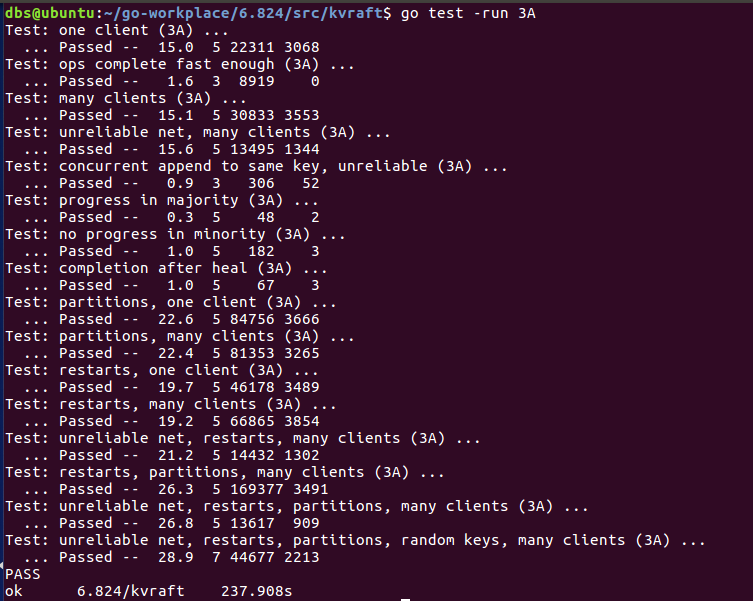
\includegraphics[width=0.8\textwidth]{./3A/3A result.png}
		\caption{3A运行结果}
	\end{figure}

	\subsection{个人总结}
	Lab3A的主要目标是实现基于Raft的键值(KV)服务器。在这个系统中,客户端通过向服务器发送请求,服务器通过底层的Raft协议来维护日志的一致性,并将操作存储在内存中。Lab3A在Raft论文中主要对应于第8节,整体实现并不复杂。该实验的目的就是在Lab2中实现的Raft服务层之上建立一个服务,并与客户端进行交互。
	
	\section{lab3-B snapshot}
	\subsection{lab2D任务分析}
	Lab 2D的任务是在之前实现的Raft算法中加入快照机制。快照机制是为了减小日志的大小,提高系统性能。
	
	\begin{itemize}
		\item 快照机制概述:快照机制是一种定期捕获整个系统状态的方法,以便在以后的某个时间点可以从这个快照中进行恢复。在Raft中,快照用于替代一系列的日志条目,从而减小存储的数据量。当日志变得很长时,通过快照机制截断部分旧的日志,只保留最新的快照以及之后的日志。
		\item 触发快照的条件: 快照机制通常不是无条件地触发的,而是在满足一些条件时才执行。可能的触发条件包括:\\
		当日志达到一定的长度或条目数量时,执行快照。\\
		当系统空闲时,执行快照。\\
		当系统中有足够多的节点已经应用了相同的日志时,执行快照。
		
		\item 实现快照的逻辑: 在Lab 2D中,需要实现将整个系统状态转化为一个快照,并将这个快照存储在持久化存储中。同时,还需要修改 Raft 的状态机,以支持从快照中进行恢复。
		
		\item 快照与日志的结合: 在实现快照机制时,需要确保与之前实现的日志复制和一致性机制协同工作。快照可能会涉及到某一时刻的状态机快照,以及之后的一系列日志条目。当节点恢复时,需要能够根据快照和日志条目还原整个系统的状态。
	\end{itemize}

	\subsection{lab3B任务分析}
	Lab 3B的任务是在Lab 3A的基础上为键值存储服务器(KV server)添加快照功能。快照机制将有助于减小系统状态的存储开销,特别是在处理大量的键值对时。以下是对Lab 3B的任务的分析:
	\begin{itemize}
	\item 快照机制的引入: 在Lab 3B中,需要修改之前实现的KV服务器,以支持快照机制。这涉及到在Raft算法中触发和处理快照的逻辑。
	
	\item 快照触发条件: 类似于Lab 2D中的Raft快照,需要确定何时触发KV服务器上的快照。触发条件可能包括:
	
	当系统中的键值对数量达到一定阈值时,执行快照。\\
	当系统空闲时,执行快照。\\
	当系统中有足够多的节点已经应用了相同的日志时,执行快照。
	
	\item 实现快照的逻辑: 修改Raft算法和KV服务器的状态机,以支持将整个系统状态转化为一个快照,并将快照存储在持久化存储中。此外,需要考虑如何在节点恢复时正确加载和应用快照。
	
	\item 与日志的交互: 确保快照机制与之前实现的Raft算法中的日志复制和一致性机制协同工作。快照可能会涉及到某一时刻的状态机快照,以及之后的一系列日志条目。在节点恢复时,需要能够根据快照和日志条目还原整个系统的状态。
	\end{itemize}

	\subsection{lab2D功能设计}
	\subsubsection{调整Raft结构体}
	由于加入了快照机制,因此需要考虑 rf.log 被修剪的情况,需要记录 lastIncludedIndex 和 lastIncludedTerm 这两个参数。这两个变量指的是在经过快照后,被修剪的最后一个 log 的 index 和 term 值。在访问 rf.log 数组中的指定 index 的 log 时,需要使用这两个变量。例如,访问 index=n 的 log,通过 rf.log 数组来访问的话,就是 rf.log[n-rf.lastIncludedIndex] ,即为 index=n 的 log。因此,将这两个变量直接添加到 raft 结构体中,利用 rf.mu 这个互斥锁方便各个协程进行互斥使用。
	\subsubsection{实现Snapshot函数}
	该函数主要由节点自己调用,用于创建一个新的快照。
	
	主要流程如下:检查要创建的快照是否已经过时,如果过时则直接返回。根据快照范围内 log 的 index,将节点自身的 log 数组进行修剪。创建好快照后,节点那些需要持久化的信息也会更新,例如 rf.log、rf.lastIncludedIndex、rf.lastIncludedTerm。然后需要将这些更新后的信息进行持久化保存。实验教程推荐使用 persister.SaveStateAndSnapshot 函数进行持久化保存快照和节点的信息。
	
	注意:在6.824中,快照的间隔是每10条 command 进行一次快照。因此,在节点提交已经确认的指令到 applyCh 进行执行时,不能获取带有 rf.mu 这个互斥锁。因为在提交指令并将该指令发送到 applyCh 执行的同时,测试脚本会调用 Snapshot 函数进行快照。但是我设计的这个函数也需要获取 rf.mu 互斥锁,那么这个节点就会进入死锁状态:无法获取 rf.mu 互斥锁进行快照,另一边需要等快照结束才能继续提交指令并执行,以及后续动作。因此,需要注意在设计中解决这个死锁问题。
	
	\subsubsection{实现InstallSnapshot功能}
	当引入快照机制后,当领导者修剪日志后,在进行日志复制时,部分跟随者可能会缺少领导者已经通过快照修剪的日志。在这种情况下,领导者需要调用该 RPC 来将自身的快照发送给相应的跟随者,以解决这个问题。
	
	需要注意的是,需要检查发送过来的快照是否是过时的,以避免旧的快照将本地新的快照覆盖,导致数据回滚。
	
	同时,节点收到快照有两种可能性:
	\begin{itemize}
	
		\item 如果发送过来的 args.LastIncludedIndex 比本节点的 lastLogIndex 大,那么节点只需删除本地的日志,并通过 args 的数据更新本地信息。此外,节点的 lastLogIndex 也应当变更为 args.LastIncludedIndex,lastLogTerm 也应当变更为 args.LastIncludedTerm。
	
		\item 如果发送过来的 args.LastIncludedIndex 比本节点的 lastLogIndex 小,那么节点只需将包括 LastIncludedIndex 在内的所有日志修剪掉即可,无需更改 lastLogIndex。

	\end{itemize}
	\par
	实验教程中指出,当一个节点收到 InstallSnapshot 时,需要将该快照信息放到 applyMsg 中,然后再放到 applyCh 中。如果只是更新节点的本地信息而不将快照信息生成一个 applyMsg 并插入到 applyCh 中,测试将会出错。
	
	因此,在生成 applyMsg 插入到 applyCh 时,需要注意上述提到的,插入到 applyCh 管道中时不能持有 rf.mu 互斥锁,以避免与测试脚本调用 snapshot 函数时发生死锁。
	
	\subsubsection{调整Start函数}
	在这里的调整主要针对那些日志落后的跟随者需要进行 InstallSnapshot 的情况。
	
	需要注意的是,在 start 函数中存在一个循环,尝试发送 sendAppendEntries 给跟随者进行日志复制。在每次循环中都需要释放并重新获取锁。重新获取锁后,节点本身的状态可能发生了更新。在2D实验中,需要额外考虑的一个状态更新是通过快照修剪了 rf.log。在发送完 sendAppendEntries 后,重新获取锁之前,还需要检查 rf.lastIncludedIndex 是否发生了变化,否则对 rf.log 进行任何访问前都需要检查 rf.lastIncludedIndex 是否改变,以避免错误。
	
	存在一种情况,当领导者尝试给跟随者进行日志复制以寻找匹配点时,进入下一次循环时,发现领导者已创建了快照,rf.log 经过修剪,nextIndex 已经小于 rf.lastIncludedIndex 即匹配点必然处于快照中,此时直接发送快照。
	
	此外,在领导者给跟随者发送快照后,更新了跟随者的状态后,领导者本地对该跟随者的状态记录也需要更新,rf.matchIndex 和 rf.nextIndex 都需要更新。
	
	在正常情况中,当领导者发送给跟随者,然后进行寻找日志复制的匹配点时,同样需要对 nextIndex 进行递减寻找。如果发现 nextIndex - 1 - rf.lastIncludedIndex == 0 且 rf.lastIncludedInex != 0,说明领导者本地的第一个日志也不是匹配点,领导者创建过快照对 rf.log 进行过修剪。在这种情况下,还需要查看快照中的最后一个日志是否匹配,若不匹配,则需要先发送快照来解决那些过于落后的日志,后续再发送本地有的日志给跟随者。
	
	在 Start 函数中,当碰到 nextIndex - 1 - rf.lastIncludedIndex == 0 的情况,这种边缘情况,就需要考虑到快照对 rf.log 进行修剪的情况。
	
	同时,在 Start 函数中,本地对那些已经提交的 msg 进行执行,并将 msg 插入到 applyCh 管道中时,务必不能持有 rf.mu 这个互斥锁,否则会导致死锁。
	
	\subsection{lab3B功能设计}
	\subsubsection{修改executeThread函数}
	这个函数启动一个线程,实时监控 applyCh 中已完成共识的请求,并立即执行这些请求。首先,通过 command.SnapshotValid 判断请求是否是执行快照的 applyMsg 的特殊消息。如果是,解码其中的信息并进行恢复。
	
	若不是执行快照的消息,则通过类型断言将 interface{} 类型转换为 Op 类型,获取 command 中的信息并执行其中的操作。在每次请求执行结束后,执行 kv.cond.Broadcast() 进行广播,唤醒等待请求执行结果的线程,使它们返回执行结果给客户端。
	
	此外,由于检测重复请求的机制,需要将已完成请求的 ID 插入队列中进行保存。在实验中,设计的队列长度为 5,保存最近执行的 5 条请求的 ID。当进行保存数据时进行快照时,将队列指定的 5 个请求和数据库的状态保存为快照。
	
	Lab3B 要求实现快照机制,触发快照的条件是当 Raft 传递给 persister.SaveRaftState() 函数进行持久化状态的数据大小超过 maxraftstate 时。但是,快照动作由 kvserver 发起,但该线程无法访问 kv.rf.persister 对象的任何信息,因为该对象是小写开头,是私有属性。因此,需要在 Raft 中设计两个接口供 kvserver 调用 persister.RaftStateSize(),以获取 Raft 当前的持久化数据大小。
	
	设计的接口名为 GetStateSizeAndSnapshotIndex(),该函数将返回 Raft 当前持久保存的数据大小以及当前快照中的日志索引值,即 lastIncludedIndex。
	
	之所以需要 lastIncludedIndex,是因为存在一种特殊情况,即一个节点在断连很长时间后,再次连接后,领导者会向这个跟随者发送大量的日志。此时,跟随者进行持久化时,数据量大小必然超过 maxraftstate。然而,该节点的 kvserver 在执行第一个请求后发现数据量太大就会立即进行快照,即使仅执行了一条请求,那么快照仅会减少一个单位的 rf.log 大小,数据量仍然大于 maxraftstate。后续每执行一条命令都会触发一次快照,这就会出现问题。因此,需要确保进行快照时,距离上次快照的状态至少相差 20 个日志,即至少执行 20 条请求,才能再次执行快照。
	
	\subsubsection{修改StartKVServer函数}
	一个 KVserver 在启动时必须检查是否存在快照,如果有快照,则需要恢复快照中的状态。因此,我们需要获取 Raft 中的快照数据信息。我在Raft里面设计了 GetSnapshot() 接口以供 KVserver 调用以获取快照的数据大小,如果有快照,则数据大小不为 0。
	
	\subsection{lab2D代码实现}
	\begin{itemize}
		\item 调整Raft结构体
		\begin{figure}[H]
			\centering
			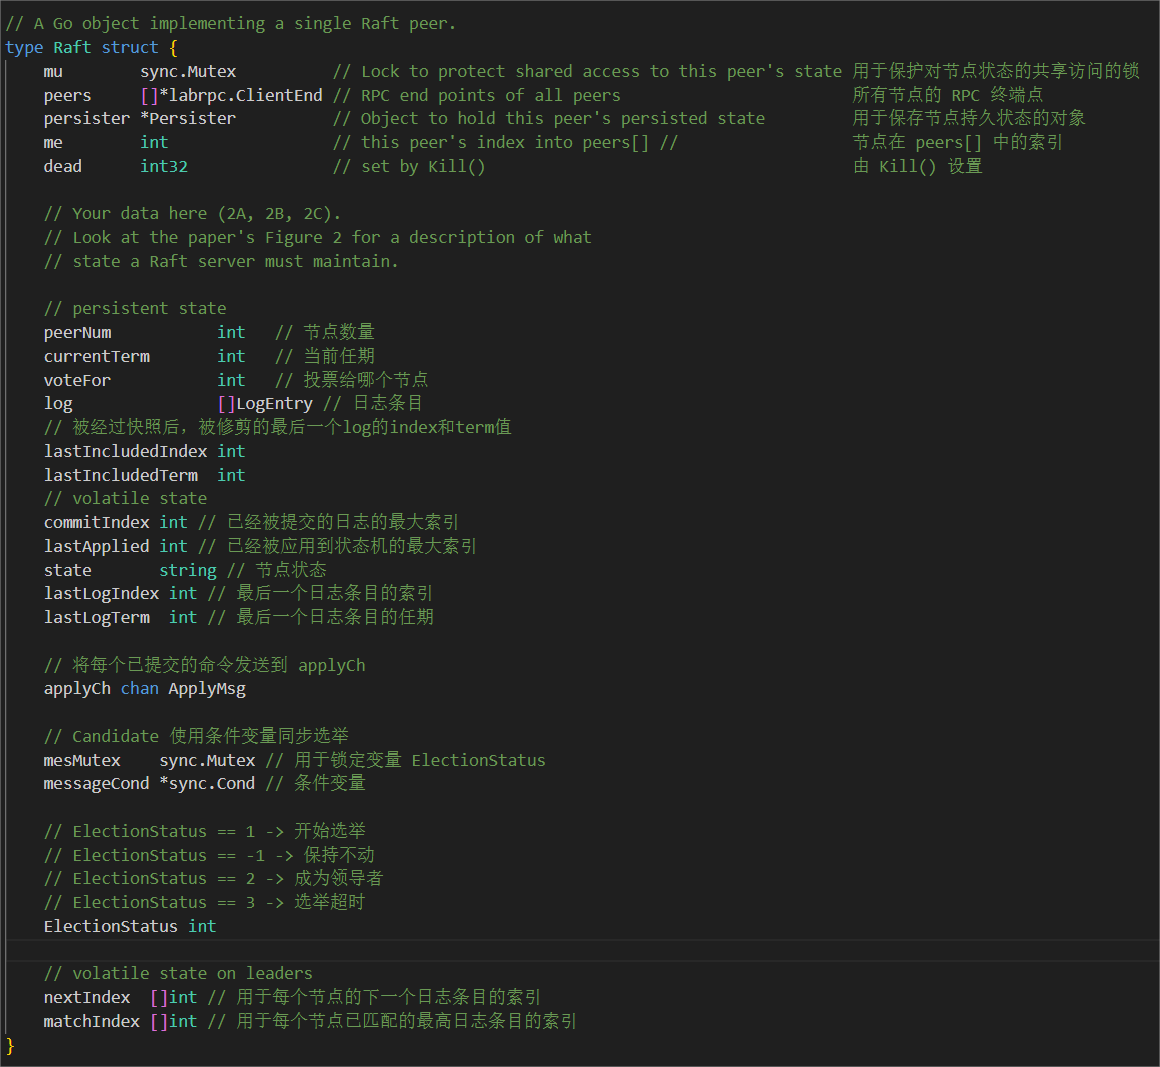
\includegraphics[width=0.8\textwidth]{./2D/Raft.png}
			\caption{Raft结构体}
		\end{figure}
		\item 实现Snapshot函数
		\begin{figure}[H]
			\centering
			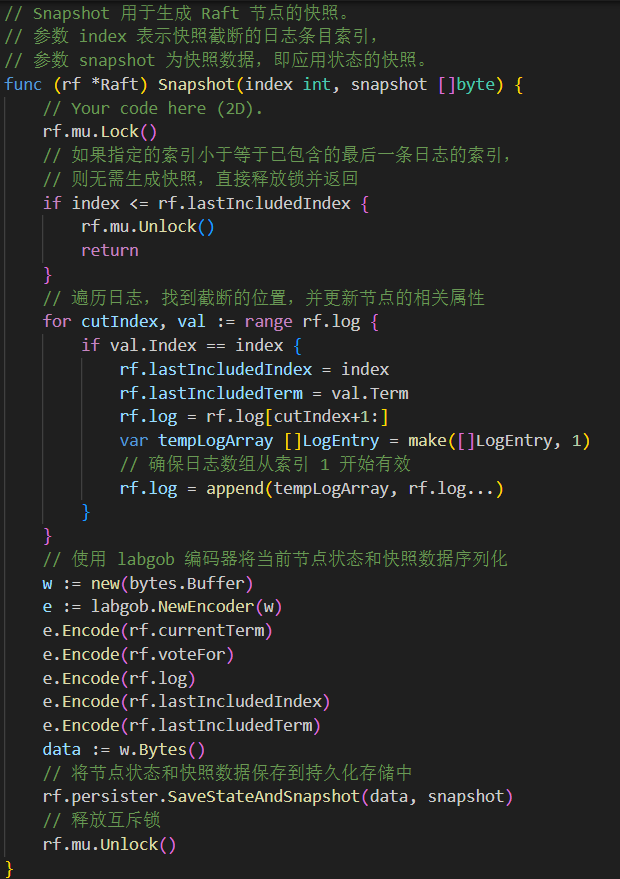
\includegraphics[width=0.8\textwidth]{./2D/Snapshot.png}
			\caption{Snapshot函数}
		\end{figure}
		\item 实现InstallSnapshot功能
		\begin{figure}[H]
			\centering
			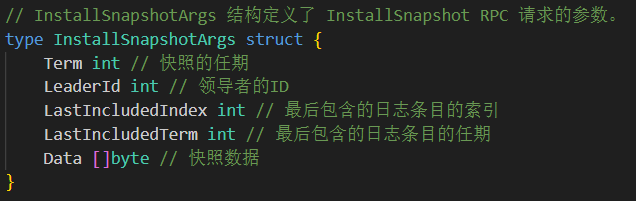
\includegraphics[width=0.8\textwidth]{./2D/InstallSnapshotArgs.png}
			\caption{InstallSnapshotArgs结构体}
		\end{figure}
		\begin{figure}[H]
			\centering
			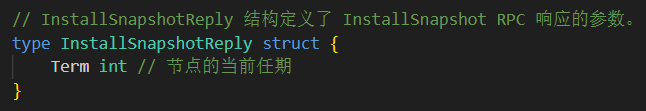
\includegraphics[width=0.8\textwidth]{./2D/InstallSnapshotReply.png}
			\caption{InstallSnapshotReply结构体}
		\end{figure}
		\begin{figure}[H]
			\centering
			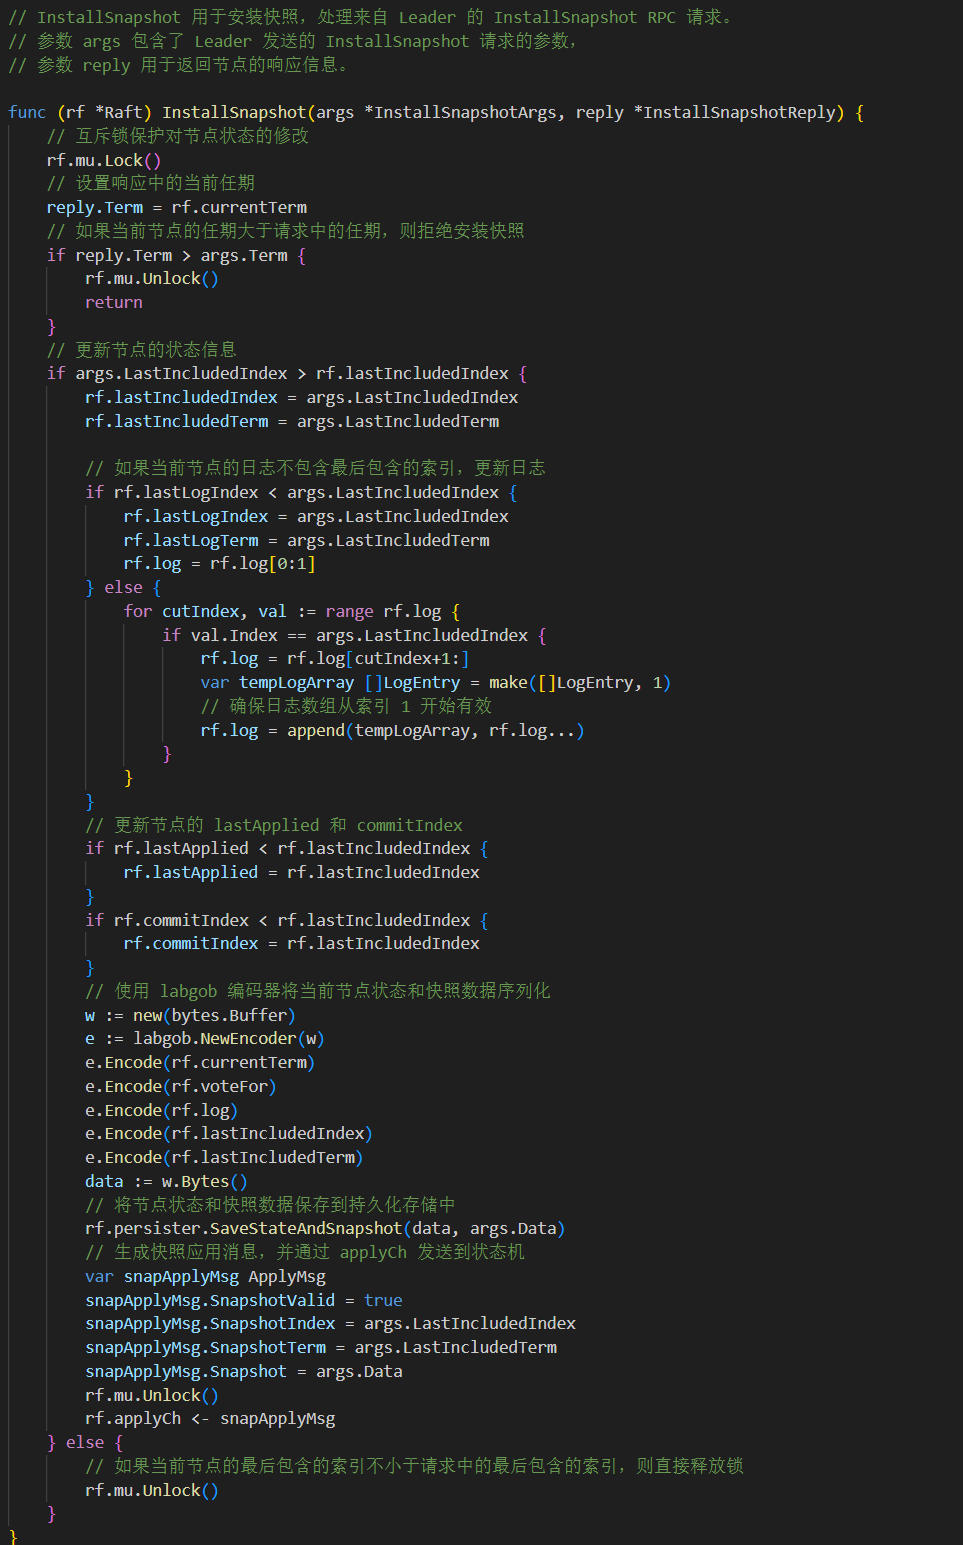
\includegraphics[width=0.8\textwidth]{./2D/InstallSnapshot.png}
			\caption{InstallSnapshot函数}
		\end{figure}
		\item 调整Start函数
		\begin{figure}[H]
			\centering
			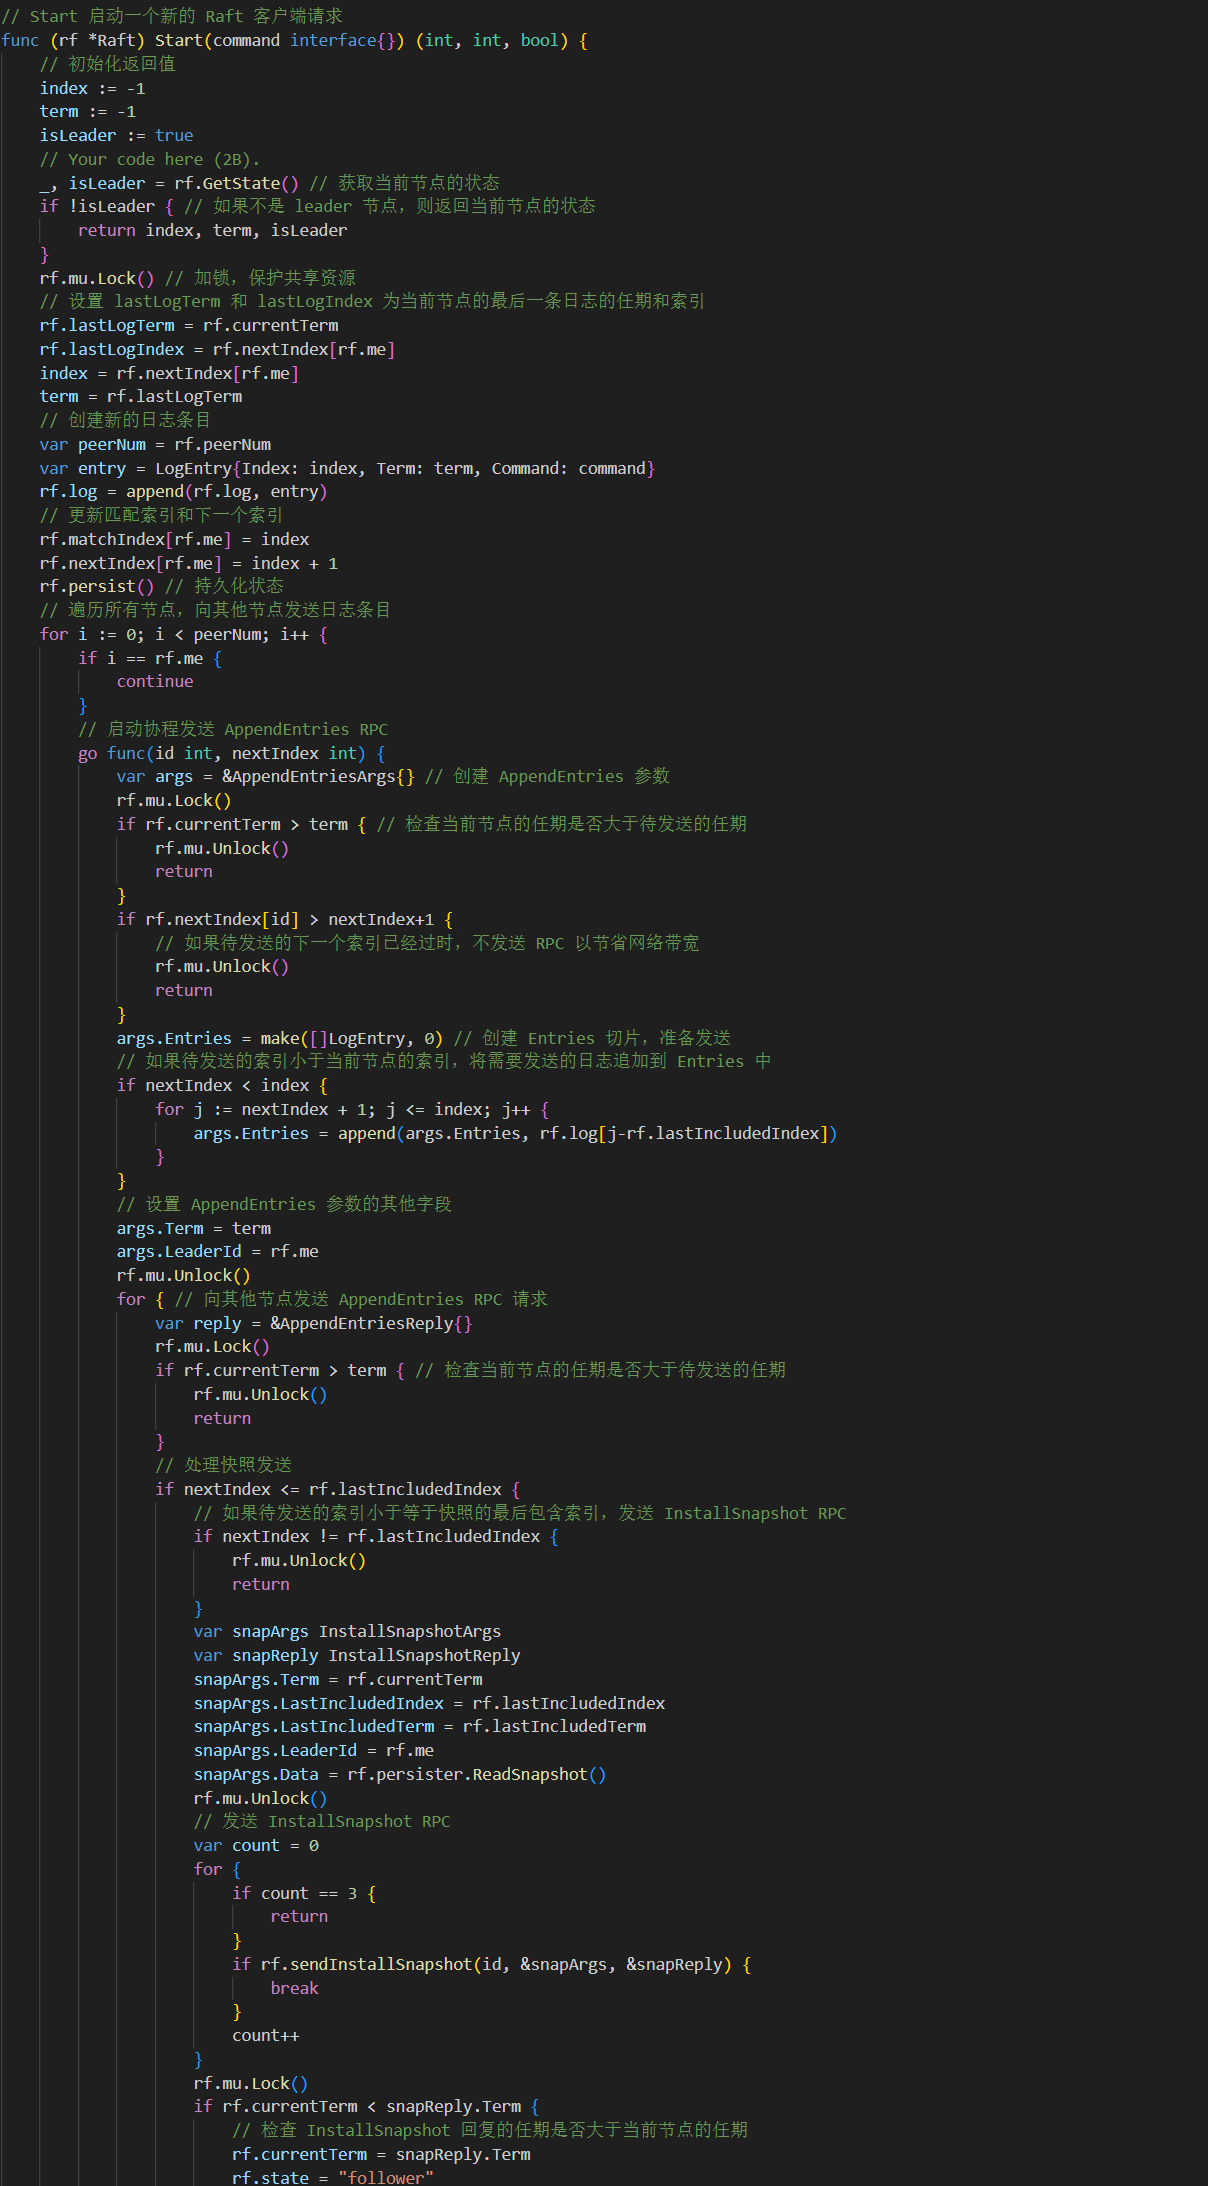
\includegraphics[height=1\textheight]{./2D/Start1.png}
		\end{figure}
		\begin{figure}[H]
			\centering
			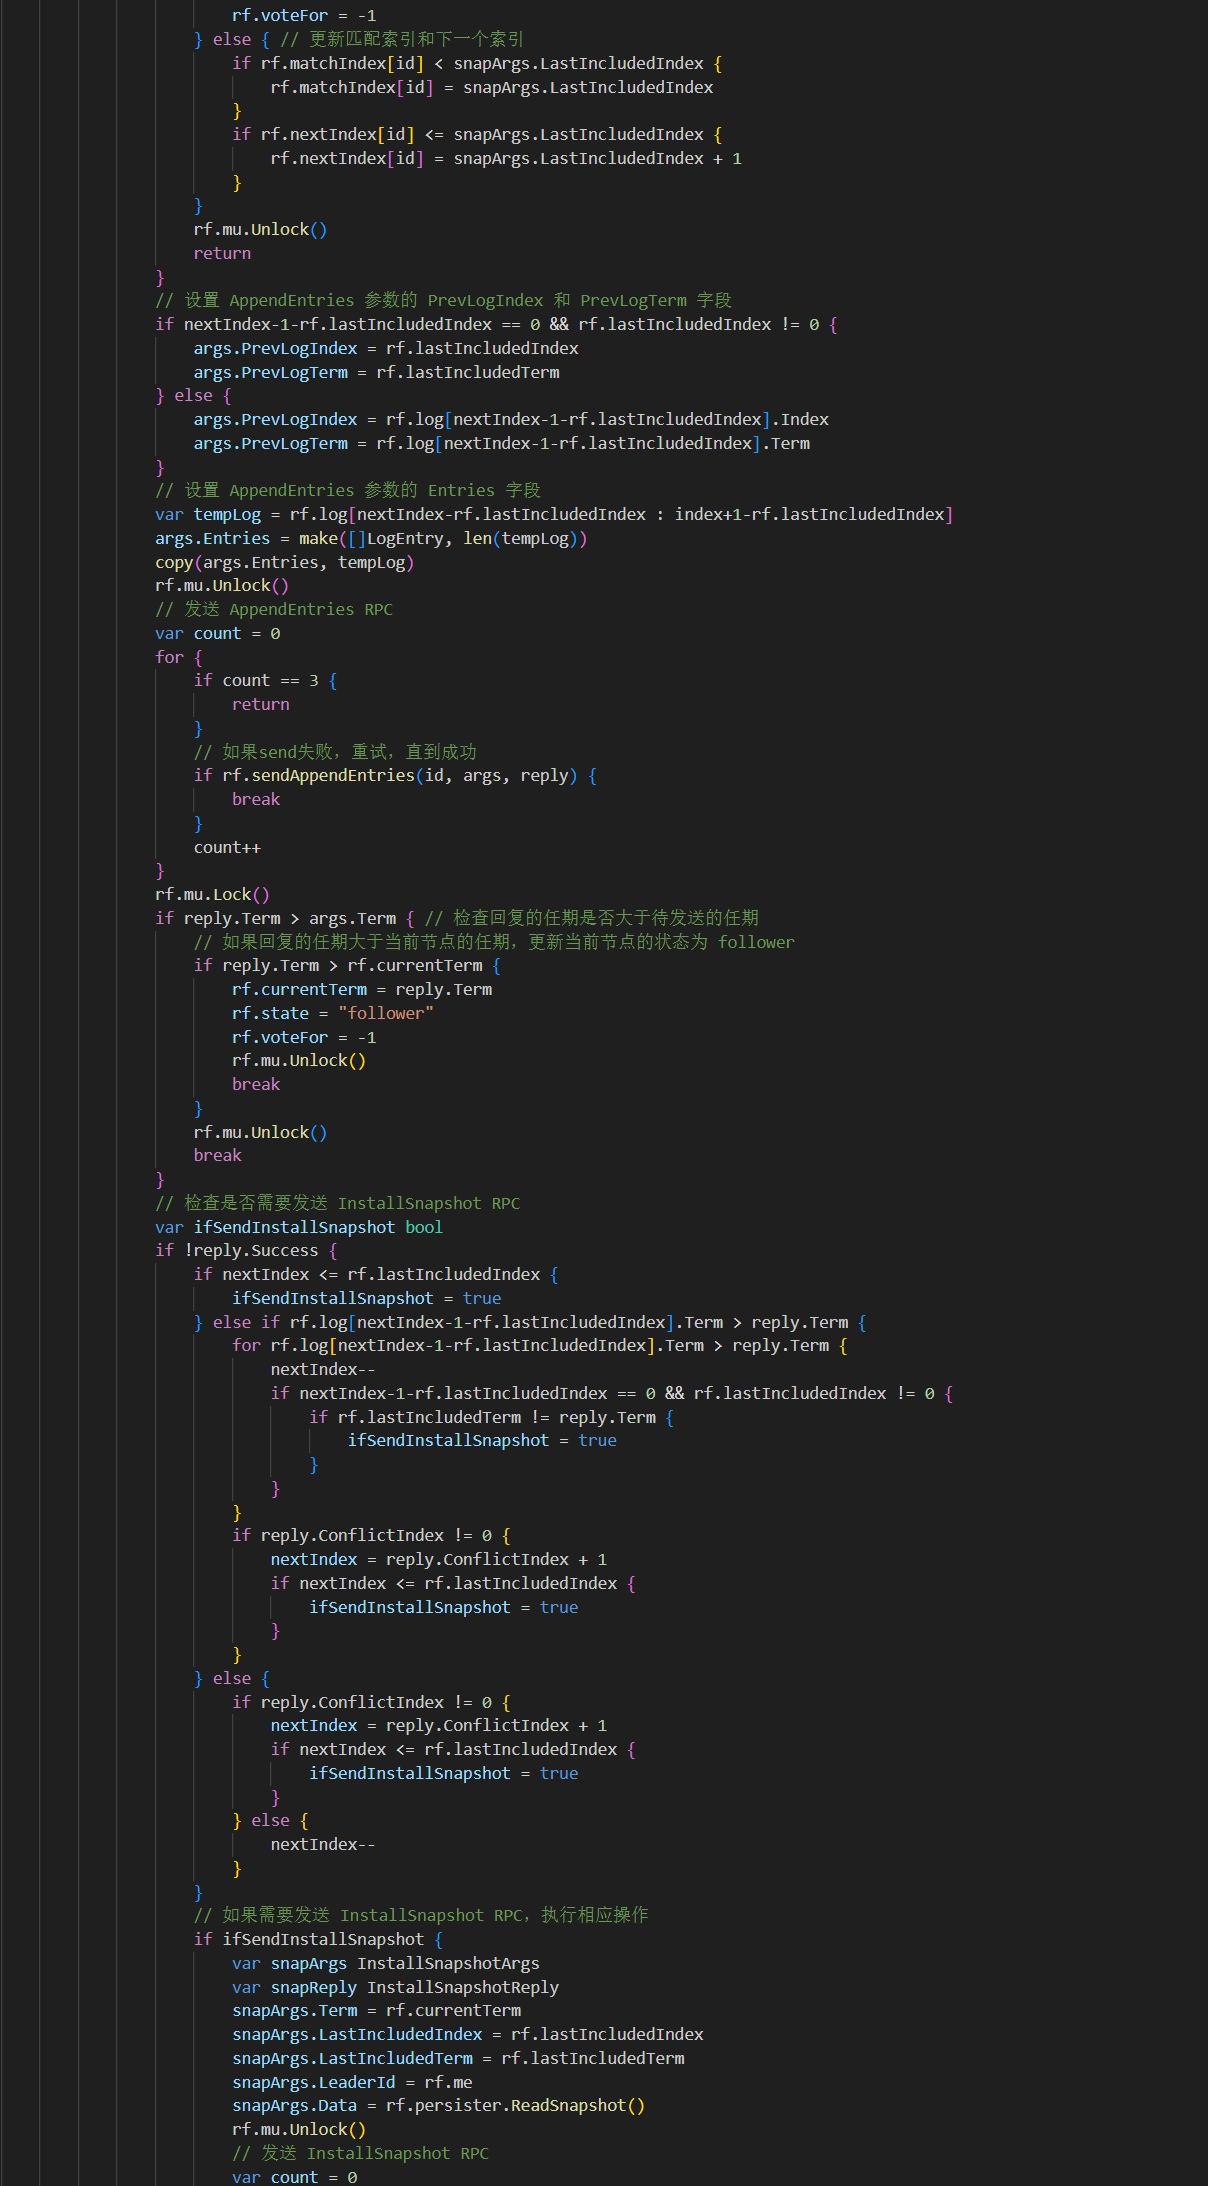
\includegraphics[height=1\textheight]{./2D/Start2.png}
		\end{figure}
		\begin{figure}[H]
			\centering
			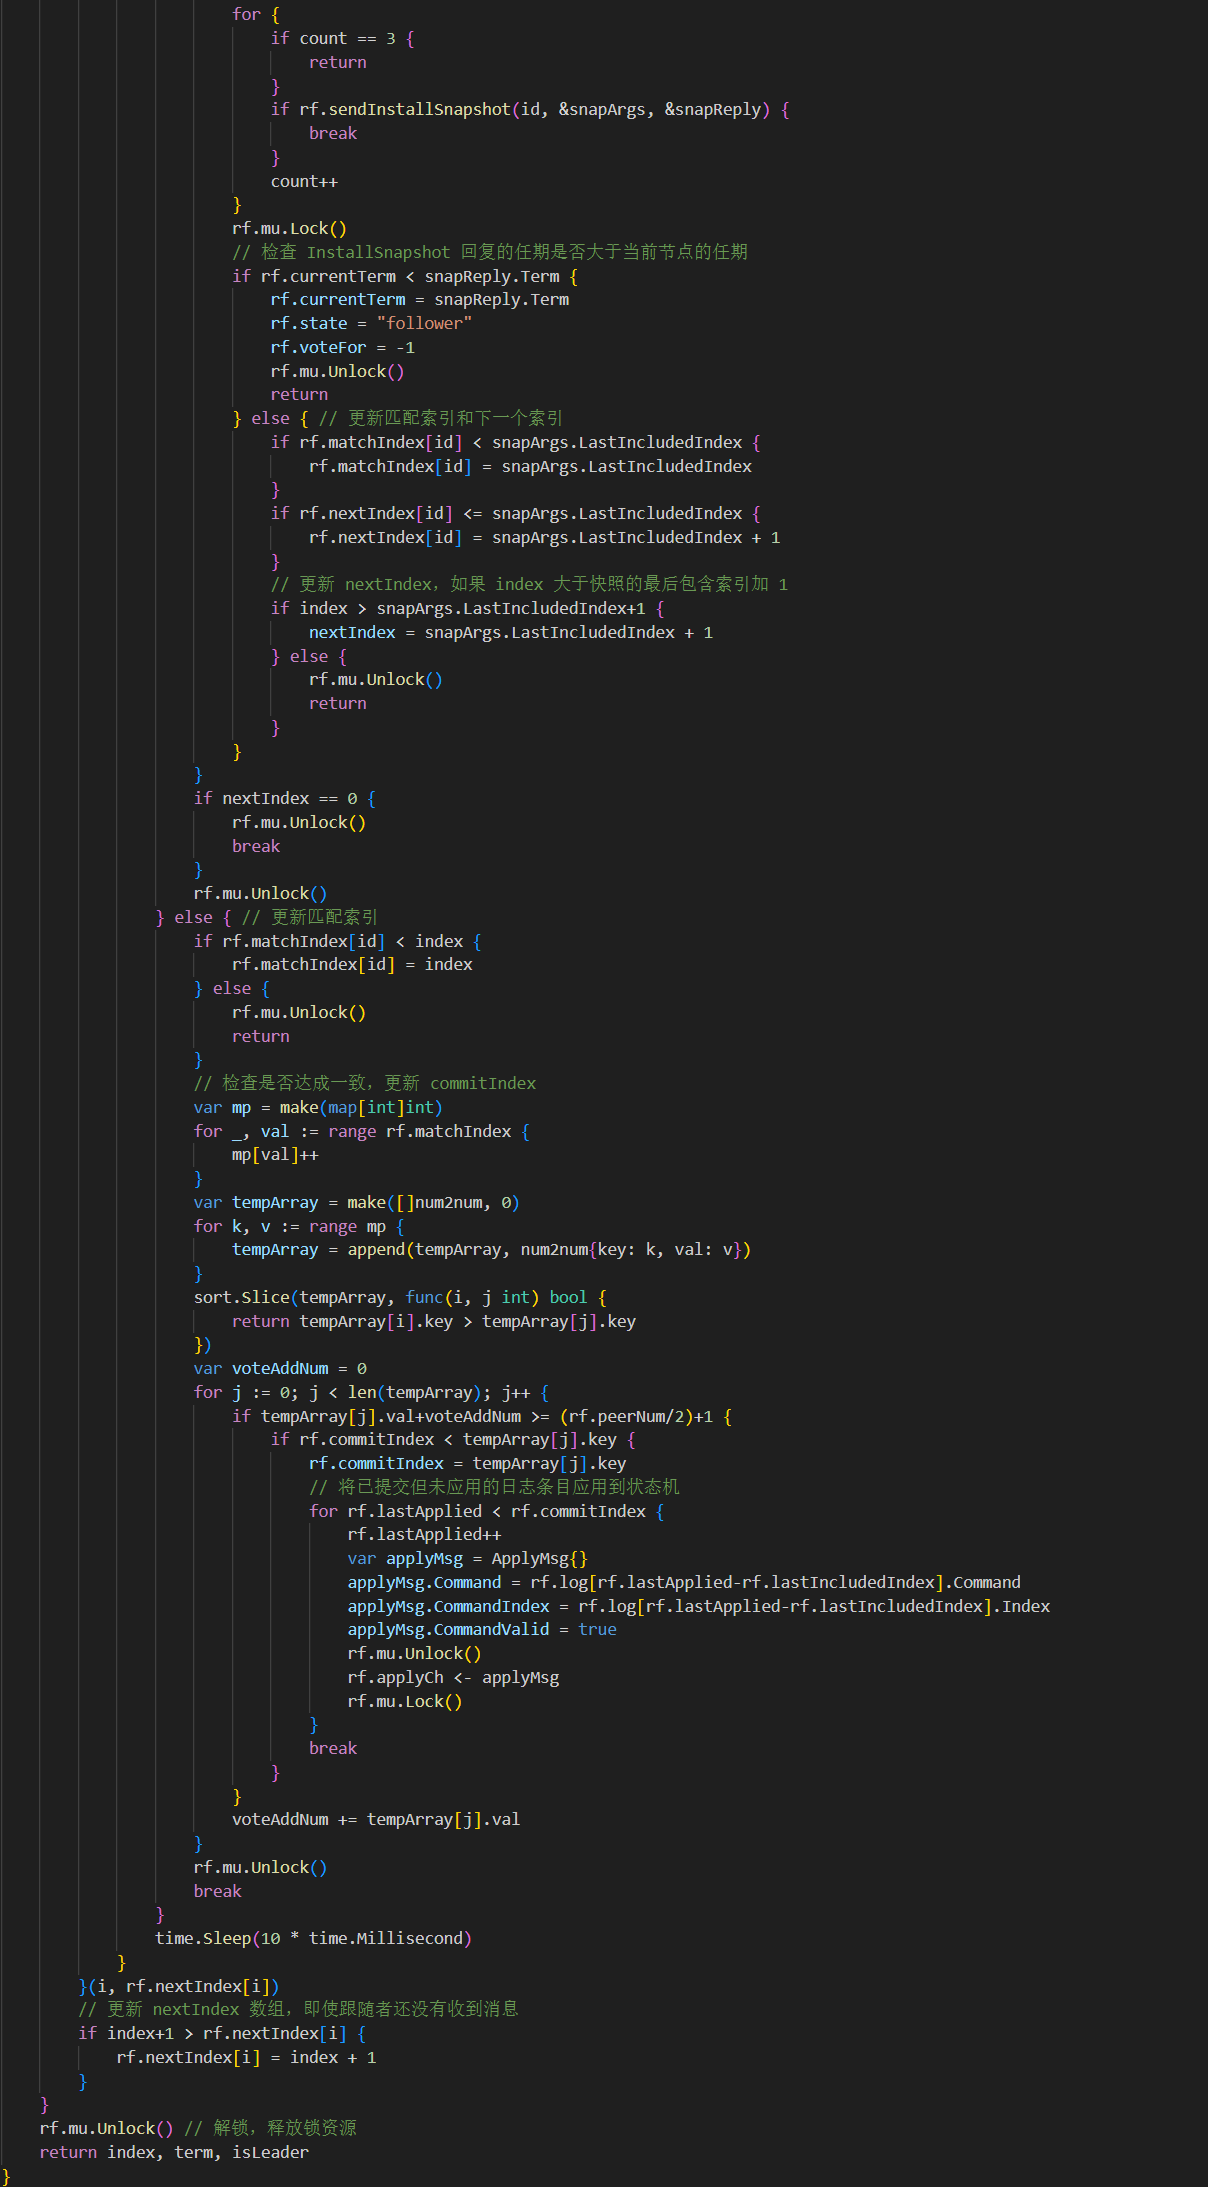
\includegraphics[height=0.95\textheight]{./2D/Start3.png}
			\caption{Start函数}
		\end{figure}
	\end{itemize}

	\subsection{lab3B代码实现}
	\begin{itemize}
		\item 修改executeThread函数
		\begin{figure}[H]
			\centering
			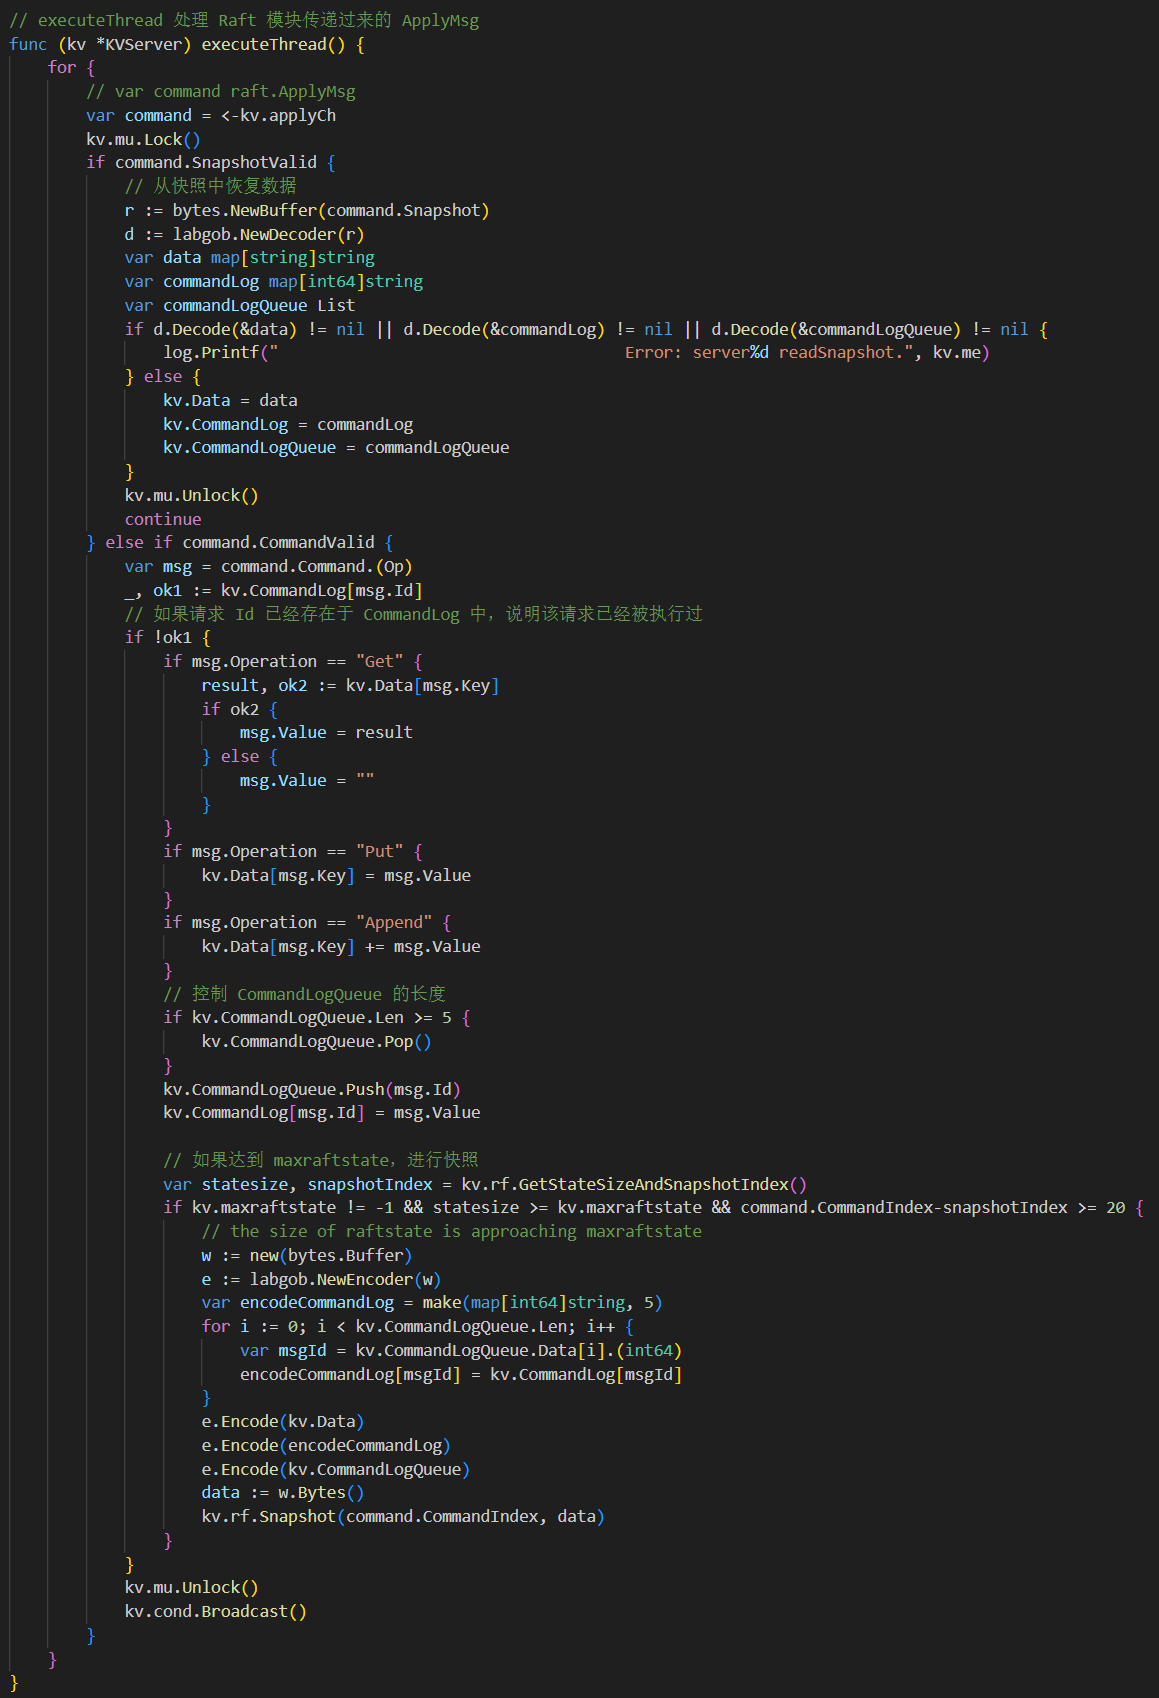
\includegraphics[height=0.85\textheight]{./3B/executeThread.png}
			\caption{executeThread函数}
		\end{figure}
		\item 修改StartKVServer函数
		\begin{figure}[H]
			\centering
			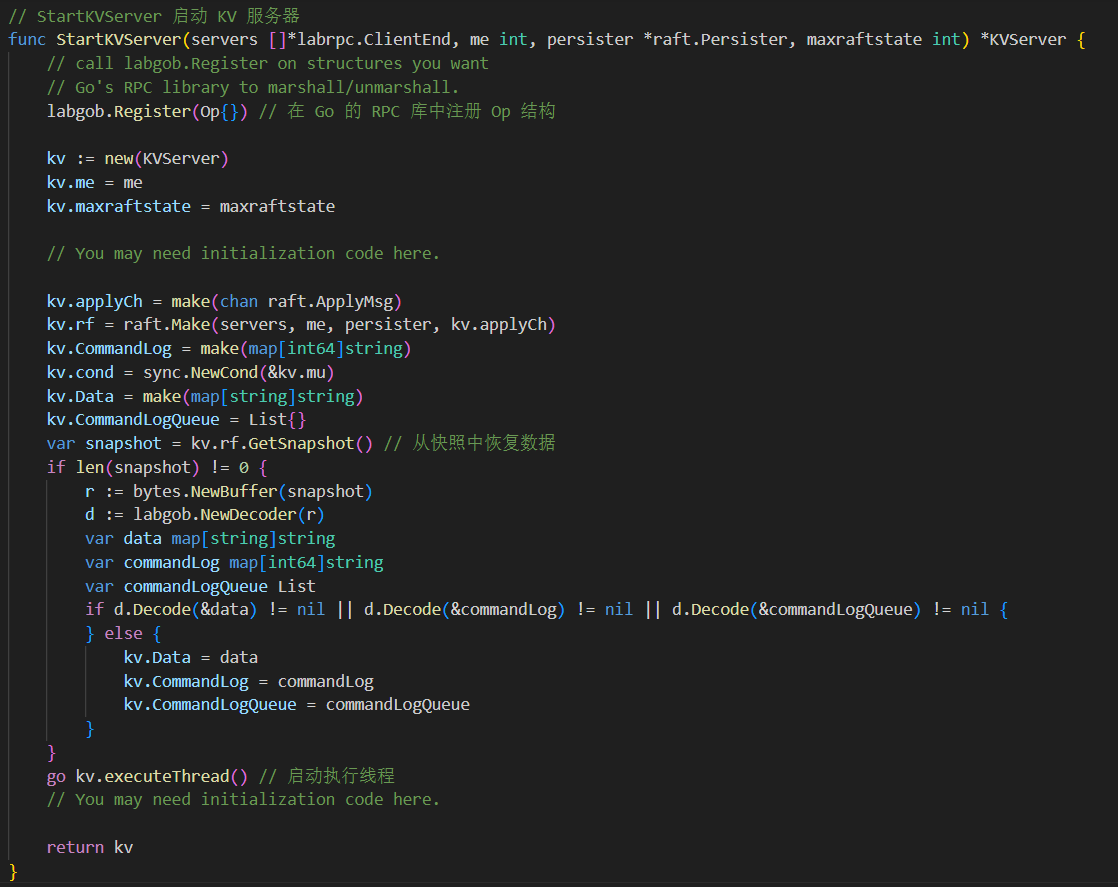
\includegraphics[width=0.8\textwidth]{./3B/StartKVServer.png}
			\caption{StartKVServer函数}
		\end{figure}
	\end{itemize}

	\subsection{测试结果}
	\begin{figure}[H]
		\centering
		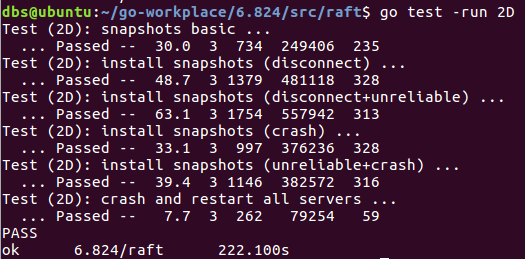
\includegraphics[width=0.8\textwidth]{./2D/2D result.png}
		\caption{2D运行结果}
	\end{figure}
	\begin{figure}[H]
		\centering
		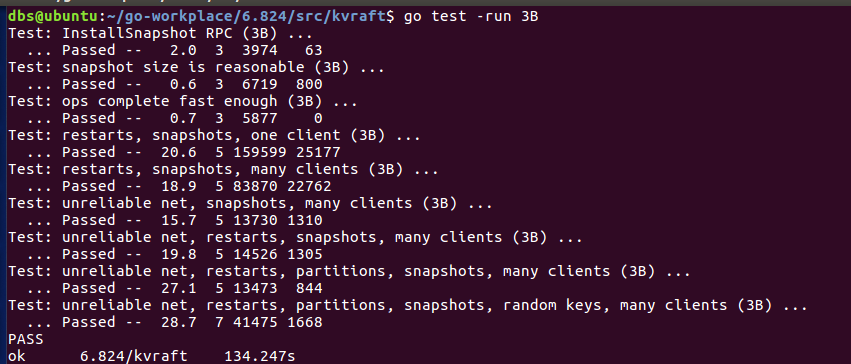
\includegraphics[width=0.8\textwidth]{./3B/3B result.png}
		\caption{3B运行结果}
	\end{figure}
	\subsection{个人总结}
	这个阶段就是引入了一个快照机制。然而,要成功实现这一机制,必须深入了解实验中快照是在何时以及如何进行的,否则就会遇到各种问题。例如,在测试Lab2D的过程中,我突然发现learer发生了死锁,测试结果还显示lastapplied的index值与commandIndex值不匹配等问题。
	
	Lab2D的代码修改范围相当大,因为涉及到了rf.log的索引值的修改以及log replication的运行逻辑的调整。在编写Lab2D的过程中,感觉就像以往的实验一样,运行测试,查找bug,然后打补丁。
	
	相比之下,Lab3B的任务相对简单。首先,在当前储存的日志数量大于maxraftstate时,需要调用snapshot()函数,并传入需要保存的持久化数据。其次,在启动KV服务器时,需要读取可能存在的快照数据。
	
	\section{心得体会}
	lab3比lab2更加自由一点,主要是没有可供参考的论文,也没有丰富的资料可供查询,同时调试的难度也明显提升。尽管如此,整个系统的实现思路基本上是一脉相承的,并没有太多自行发挥的空间。在查阅了一些网上的博客之后,我发现虽然不同的实现方式各有不同,但设计思路却是相似的。
	
	相对于Lab2,Lab3的代码复杂性并不高,因此代码量也较为有限。在实现过程中,我尽量避免修改raft的源码,因为一旦对raft源码进行修改,可能会带来不必要的麻烦,尤其是在出现bug时修改起来更为头疼。这种小心谨慎的策略帮助我有效地应对了潜在的问题。
	
	整个Lab 3的实践是我在分布式系统领域深入学习的重要一步。实现基于Raft的键值存储服务是这个实验的重要组成部分。这一部分让我学到了如何设计和构建一个分布式系统,考虑节点的协同工作、一致性维护以及客户端与服务器之间的通信。在这个实验中,我不仅巩固了Raft一致性算法的理论知识,还通过完成构建基于Raft的分布式键值存储服务的实验,将理论知识应用到实际场景,为我在分布式系统领域的学习和实践提供了宝贵的经验。我期待着在未来的学习中继续探索分布式系统的更多方面。
	
	\section{参考资料}
	\begin{itemize}
		\item MIT 6.824 学习(二)【Raft】 : https://blog.csdn.net/weixin\_48922154/article/details/123956614
		\item MIT6.824 Lab3实现与踩坑 : https://blog.csdn.net/darkLight2017/article/details/122587599
		\item MIT 6.824 Lab3 翻译(Key/Value Server Base on Raft) :https://zhuanlan.zhihu.com/p/267685488
		\item Lecture 06 - Raft1 : https://mit-public-courses-cn-translatio.gitbook.io/mit6-824/lecture-06-raft1 
		\item MIT 6.824 lab3 KVRaft : https://blog.csdn.net/Miracle\_ma/article/details/80184594
	\end{itemize}
	
\end{document}
